\section{Database Design}
The database has to store all the information in the \ac{giraf} system.
To get an overview of the entire database, an entity-relationship diagram (ER diagram) has been constructed. \autoref{fig:erdiagram} illustrates the ER diagram for the database.

\begin{figure}[hptb]
\begin{center}
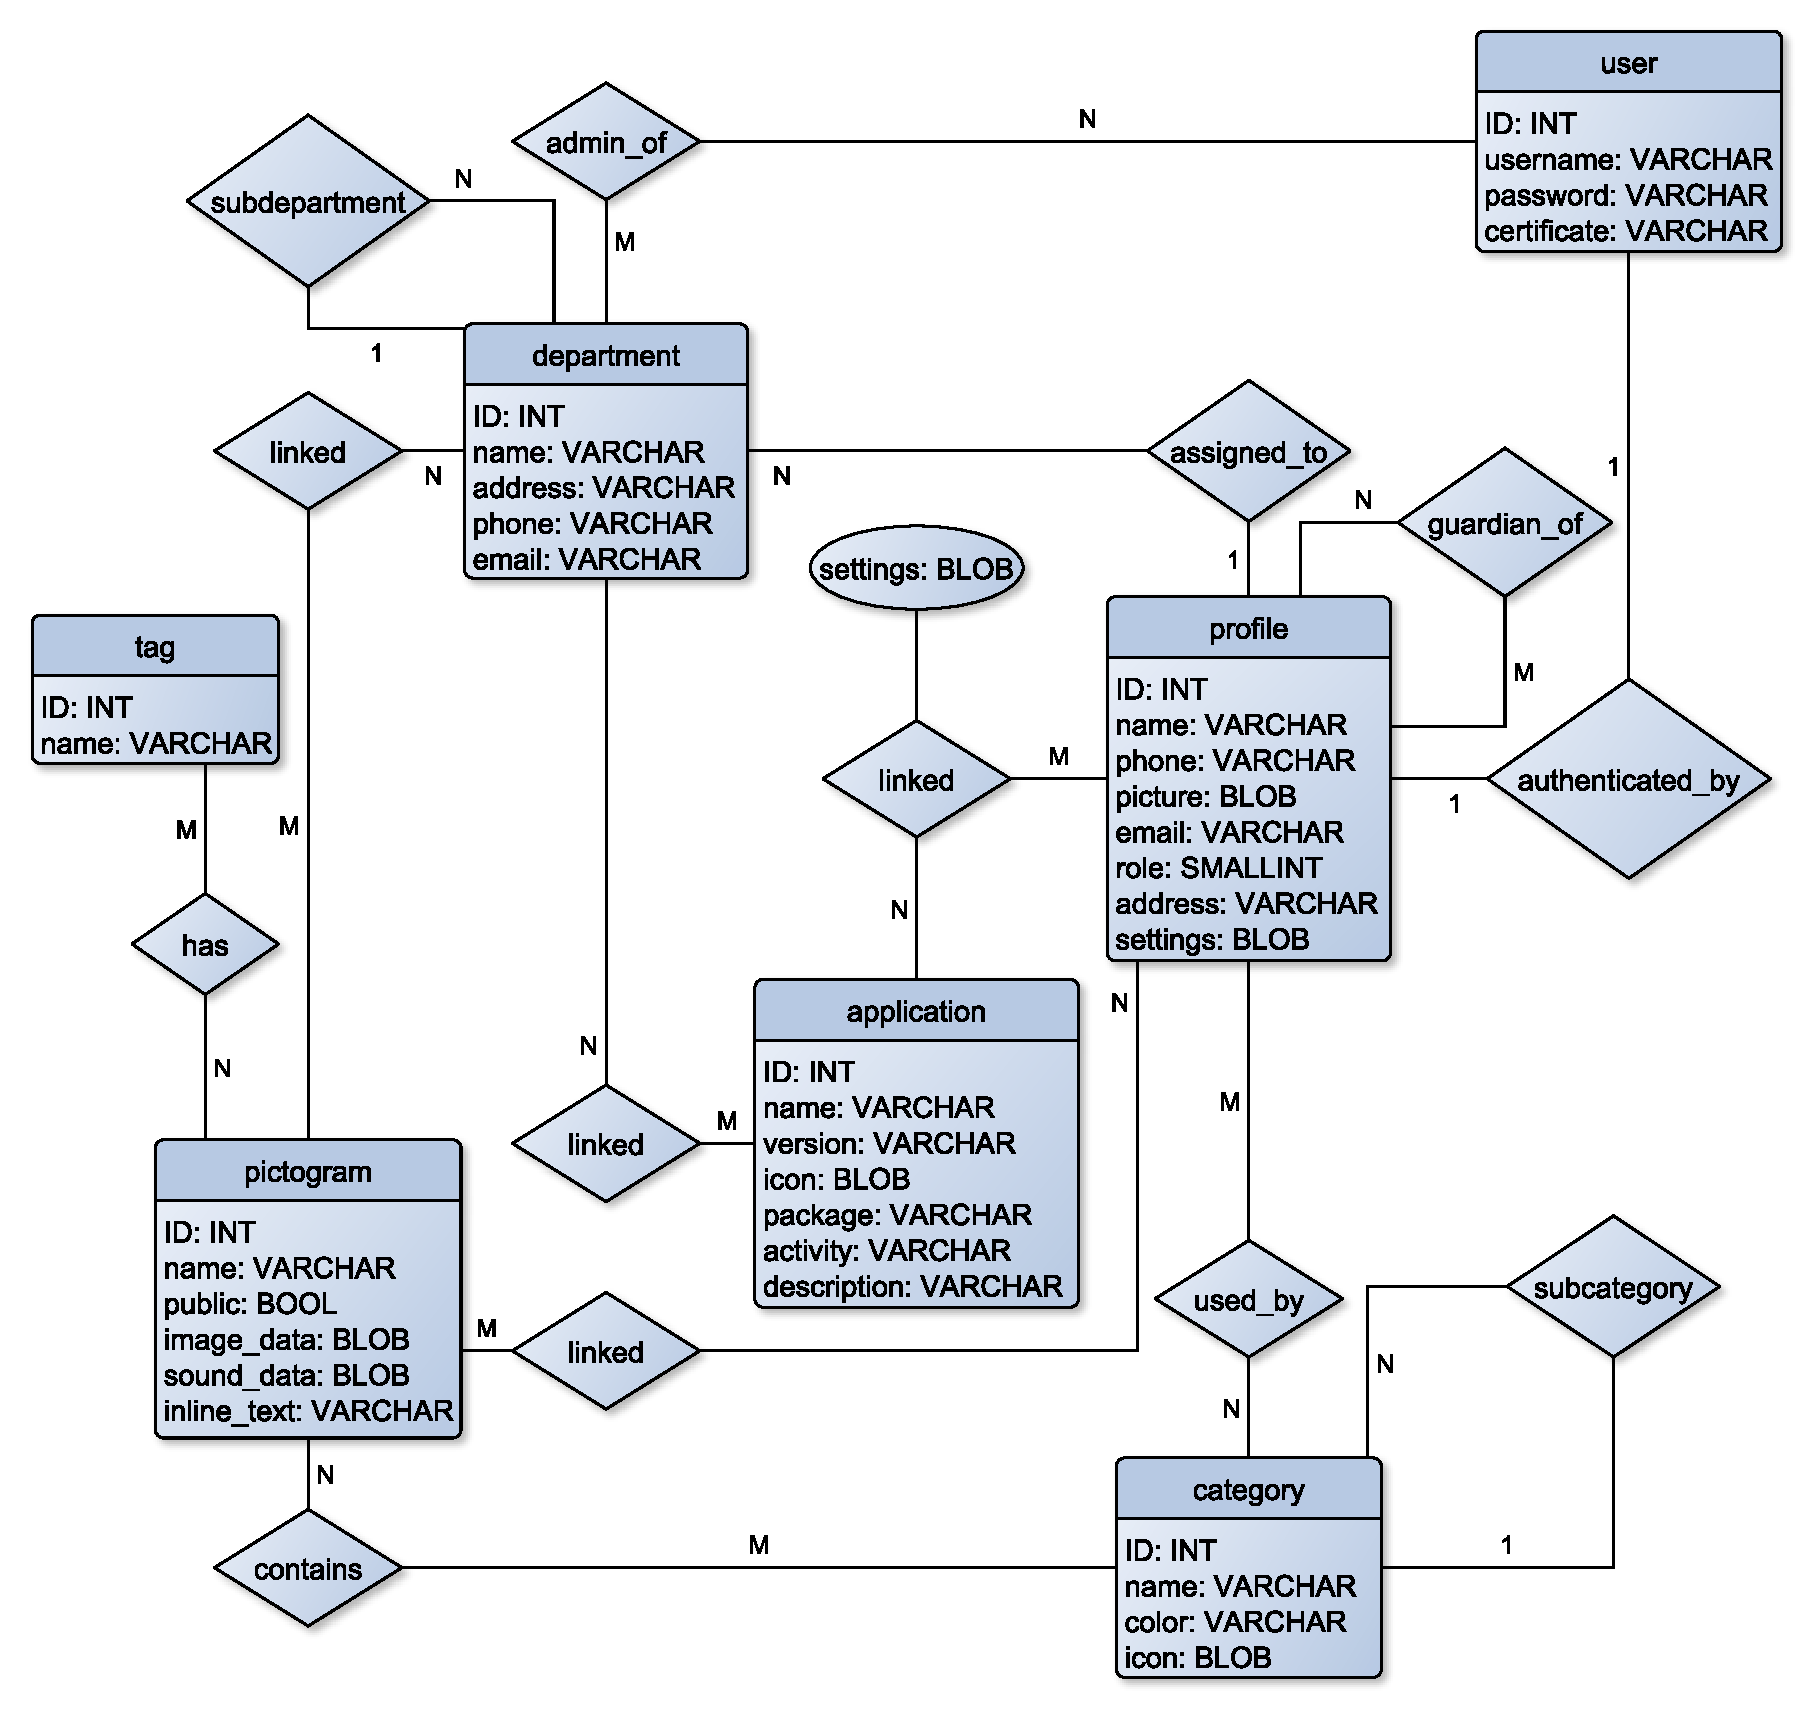
\includegraphics[width=\textwidth]{img/ER_diagram3.pdf}
\caption{ER Diagram}
\label{fig:erdiagram}
\end{center}
\end{figure}

The ER diagram uses a collection of basic objects called entities and their relationships to describe concepts in the real world and their individual relations. The group based the current diagram on the 2012 version, re-using some attributes for entities, but cleaning up relations and adding new content needed by other groups (e.g. pictogram category). 

\subsection{Profile}
The profile entity includes both children and guardians, it holds information such as name, phone number, picture, e-mail, address and role (i.e. child, parent or employee). The roles are important in determining the privileges of the account. Profiles with the parent role can only administrate their own and their children's profiles, whereas profiles with the employee role on the other hand can administrate the profiles of the parents as well as the children. 

Settings such as preferences with regards to background colour and the like, can be extremely important to an autistic person, and varies wildly from person to person, and thus these need to be stored in the database. They are saved in a blob because the data type is faster to use and because the data will not have to be manipulated through the database.

The phone number is saved as a varchar to allow users to save country codes (such as +45 for Denmark). 

It is assumed that no address is longer than 256 characters.

The \emph{guardian\_of} relationship enables one profile to be guardian of several other profiles. This is because the children should not have the authority to administrate their own pictograms and settings, they rely on a guardian to handle all of the customization in cooperation with them. 

The settings of an application are saved in the relation to the profile in order to allow different users to customize the look of the application.

\subsection{Application}
The application entity holds information such as name, version, icon, package, activity and description. 
The package attribute signifies which Android package the application is included in and the activity attribute is the main activity of the application. Applications can be associated to both departments and profiles, depending on whether the application should be accessible to a single profile or all profiles associated with the department. As previously mentioned the settings are not stored as a part of the actual application, but in the relation to the profiles. This makes it easier customize the application for each individual profile.

\subsection{Department}
The department entity contains information such as name, address, phone and email. Departments have a number of profiles assigned to it i.e. employees and children.

The fact that applications and pictograms can be associated with departments signifies, that a department can allow all users affiliated with it to have access to specific applications and pictograms related to that department. This is done to ensure that all children, parents and employees can have access to common data, e.g. a picture of the department they are associated with.

\subsection{Pictograms}
The pictogram entity contains name, public, image data, sound data and some inline text. 
Pictograms can be a mixture of image, sound and text. The \emph{public} attribute signifies whether the pictogram is public or restricted to a specific profile or department. 

As of now, the image and sound data are supposed to be stored as blobs in the database, however in a production environment these data should be stored in files on the server and a system for uploading and downloading these should be implemented. This, however, is out of scope for the current project. 

\subsubsection{Categories}
The pictograms can be arranged into categories each with its own name, colour and icon.
An example could be pictograms of various food items being put in a category named food, which could have a subcategory called breakfast that could include items such as cereal and orange juice.

\subsubsection{Tags}
Each pictogram can have a series of tags. The tags can help categorize the pictograms.

\subsection{User}
In order to distinguish the various profiles and prevent unauthorized access to sensitive information in the system some kind of user authentication is needed. The user entity holds information such as username, password and certificate.
The username and password will be used e.g. if an administrator needs to log into the system on a desktop computer. The certificate is a QR-Code that a guardian will scan with the tablet in order to log into the system. Each guardian will have their own personal QR-Code that they can use to administrate the children that they are responsible for.